TODO: write some text here. Conclusion and stuff.

- influence of the various parameters
- code too slow for realtime, but not optimized at all
- using Matlab for more than just a few hacked scripts: bad idea

\begin{figure}
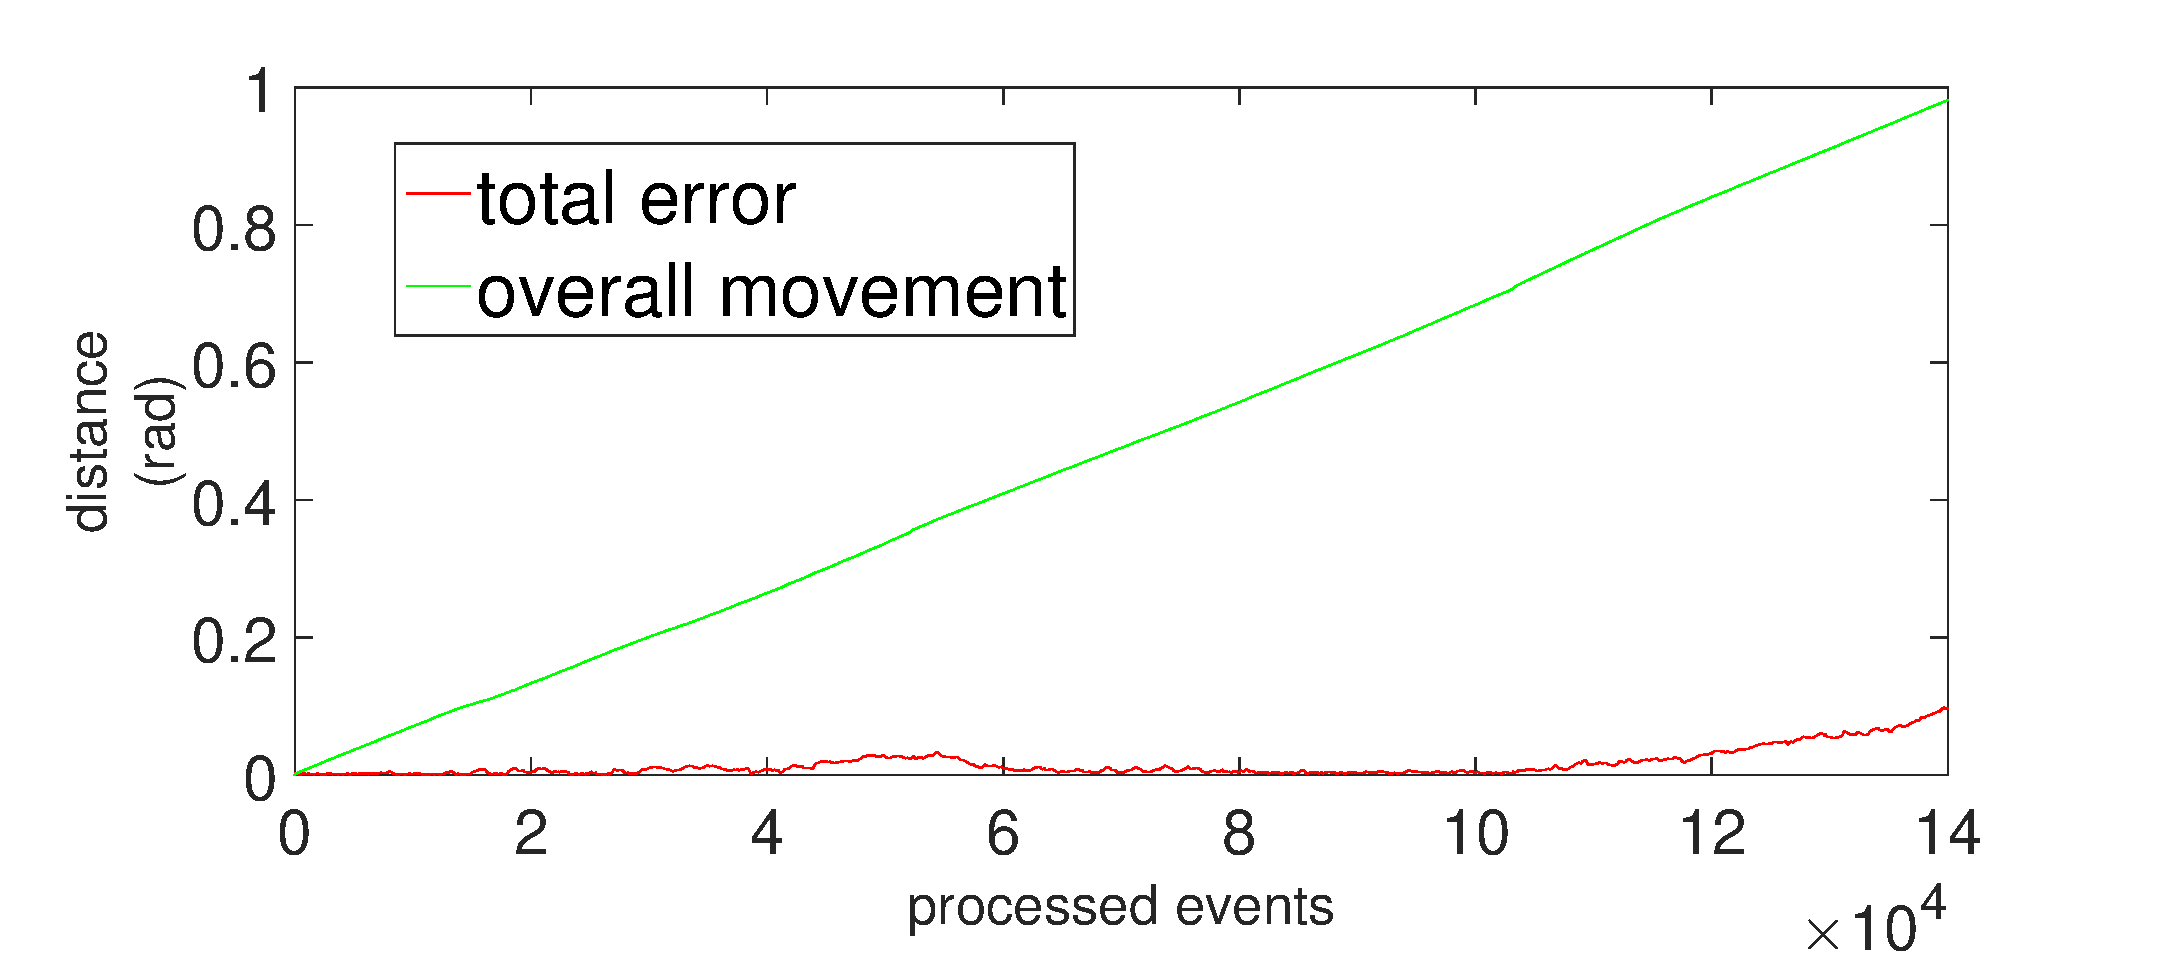
\includegraphics[width=\linewidth]{images/Tracking_error_during_reconstruction.eps}
\label{fig:tracking_error_reconstruction}
\caption{The tracking error (red) in comparison to the total travelled distance (green)
while reconstructing the map.
}
\end{figure}

\begin{figure}
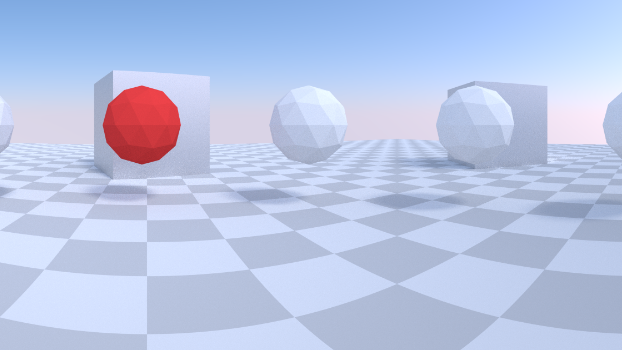
\includegraphics[width=\columnwidth]{images/zigzag_input.png}
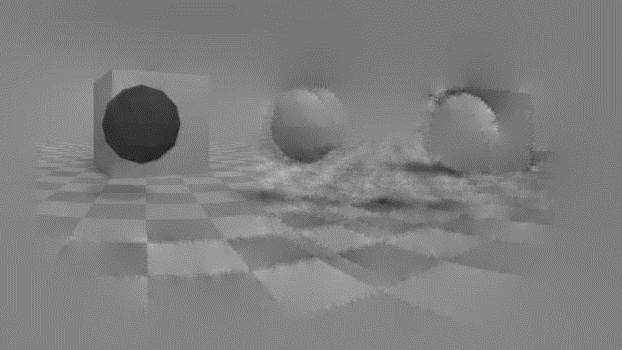
\includegraphics[width=\columnwidth]{images/zigzag_reconstruction.png}
\caption{A part of the input scene (top) and its reconstruction,
moving the camera in a large triangle waveform pattern to the right.
The area around the leftmost ball in the scene was used to initialize
the map as described in section \ref{sec:core_algorithm}.}
\label{fig:zigzag_reconstruction}
\end{figure}
